\documentclass[12pt]{article}
\usepackage[utf8]{inputenc}
\usepackage[letterpaper, portrait, margin=1in]{geometry}
\usepackage{amssymb}
\usepackage{amsmath}
\usepackage{graphicx}
\usepackage{tcolorbox}

\newcommand{\example}[1]{\noindent\textbf{Example #1\quad}}
\newcommand{\exercise}[1]{\noindent\textbf{Exercise #1\quad}}
\newcommand{\problem}[1]{\noindent\textbf{Problem #1\quad}}

\pagenumbering{arabic} % arabic, roman, Roman, alph, Alph, gobble
%\setcounter{page}{0} % sets the initial page

\setlength{\parindent}{0pt}
\setlength{\parskip}{10pt}
\setlength{\baselineskip}{15pt}
\linespread{1.2}

\font\sf = cmss10

\usepackage{fancyhdr}
\pagestyle{fancy}
\fancyhf{}
\lhead{MATH 180 Notes}
\rhead{Section 6.1: Areas Between Curves}
\rfoot{Page \thepage}
%\thispagestyle{empty}


\begin{document}


Goal: Find the area between two curves of $y = f(x)$ and $y = g(x)$.

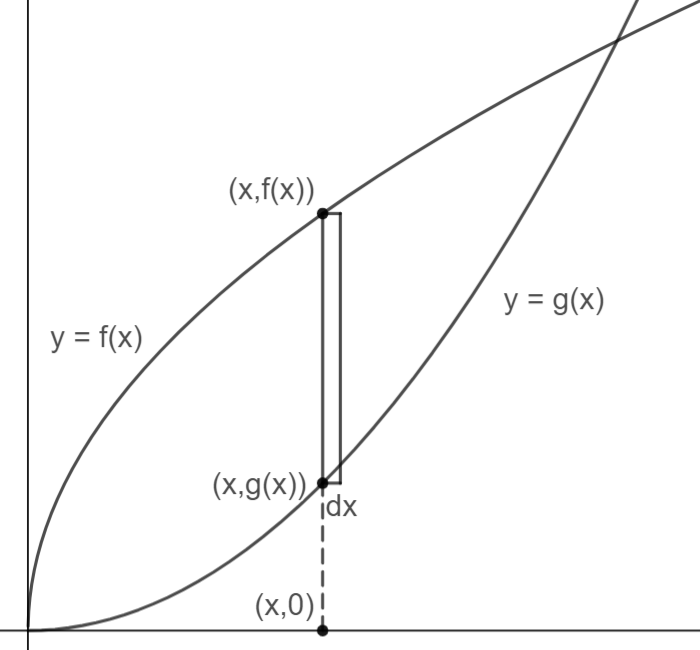
\includegraphics[scale=0.7]{math180_sec6_1_img1.png}

$$ \boxed{\quad A = \lim_{n \to \infty} \sum_{k=1}^n (f(x_k^*) - g(x_i^*))\Delta x \quad} $$

\begin{tcolorbox}
The area $A$ of the region bounded by the curves $y = f(x)$, $y = g(x)$, and the lines
$x = a$, $x = b$, where $f$ and $g$ are continuous and $f(x) \ge g(x)$ for all $x$ in $[a,b]$, is
$$ A = \int_a^b (f(x) - g(x)) \, dx $$
\end{tcolorbox}

\example{1} Find the area of the region bounded above by $y = \sqrt{x}$ and lower boundary curve is 
$y = \ln(x)$, and bounded on the sides by $x = 2$ and $x = 8$.


\begin{tabular}{ll}
\begin{tabular}{l}
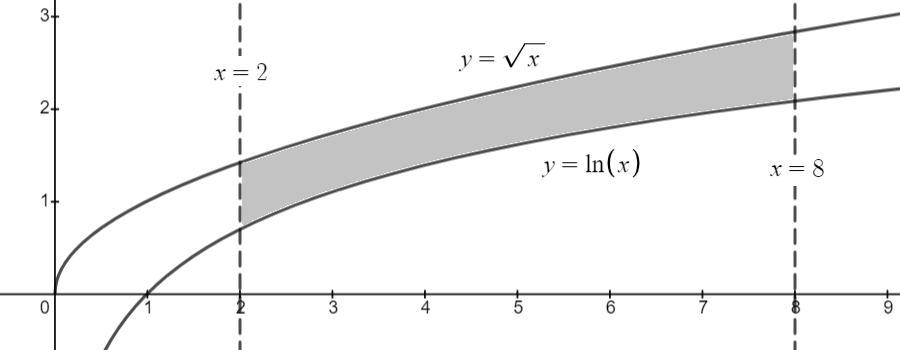
\includegraphics[scale=0.6]{math180_sec6_1_img2.png}
\end{tabular} & \begin{tabular}{l}
Note that $\sqrt{x} \ge \ln(x)$\\
for all $x$ in $[2,8]$. \\
\\
Upper function: \\
$f(x) = \sqrt{x}$ \\
Lower function: \\
$g(x) = \ln(x)$
\end{tabular}
\end{tabular}
\begin{eqnarray*}
A &=& \int_2^8 (\sqrt{x} - \ln(x)) \, dx \\
&=& \left(\frac{2}{3}x^{3/2} - (x\ln(x) - x)\right)\Bigg|_2^8 \\
&=& \frac{2}{3}(8)^{3/2} - (8\ln(8) - 8) - \left(\frac{2}{3}(2)^{3/2} - (2\ln(2) - 2)\right) \\
&=& \frac{2}{3}(8)^{3/2} - 8\ln(2^3) + 8 - \frac{2}{3}(2)^{3/2} + 2\ln(2) - 2 \\
&=& \frac{2}{3}(16\sqrt{2}) - 24\ln(2) + 6 - \frac{2}{3}(2\sqrt{2}) + 2\ln(2) \\
\end{eqnarray*}



\begin{tcolorbox}
The area between the curves $y = f(x)$ and $y = g(x)$ and between $x = a$ and $x = b$ is
$$ A = \int_a^b |f(x) - g(x)| \, dx $$
\end{tcolorbox}





















\end{document}
